\subsection{時制の持つ意味}

\begin{figure}[h]
  \centering
  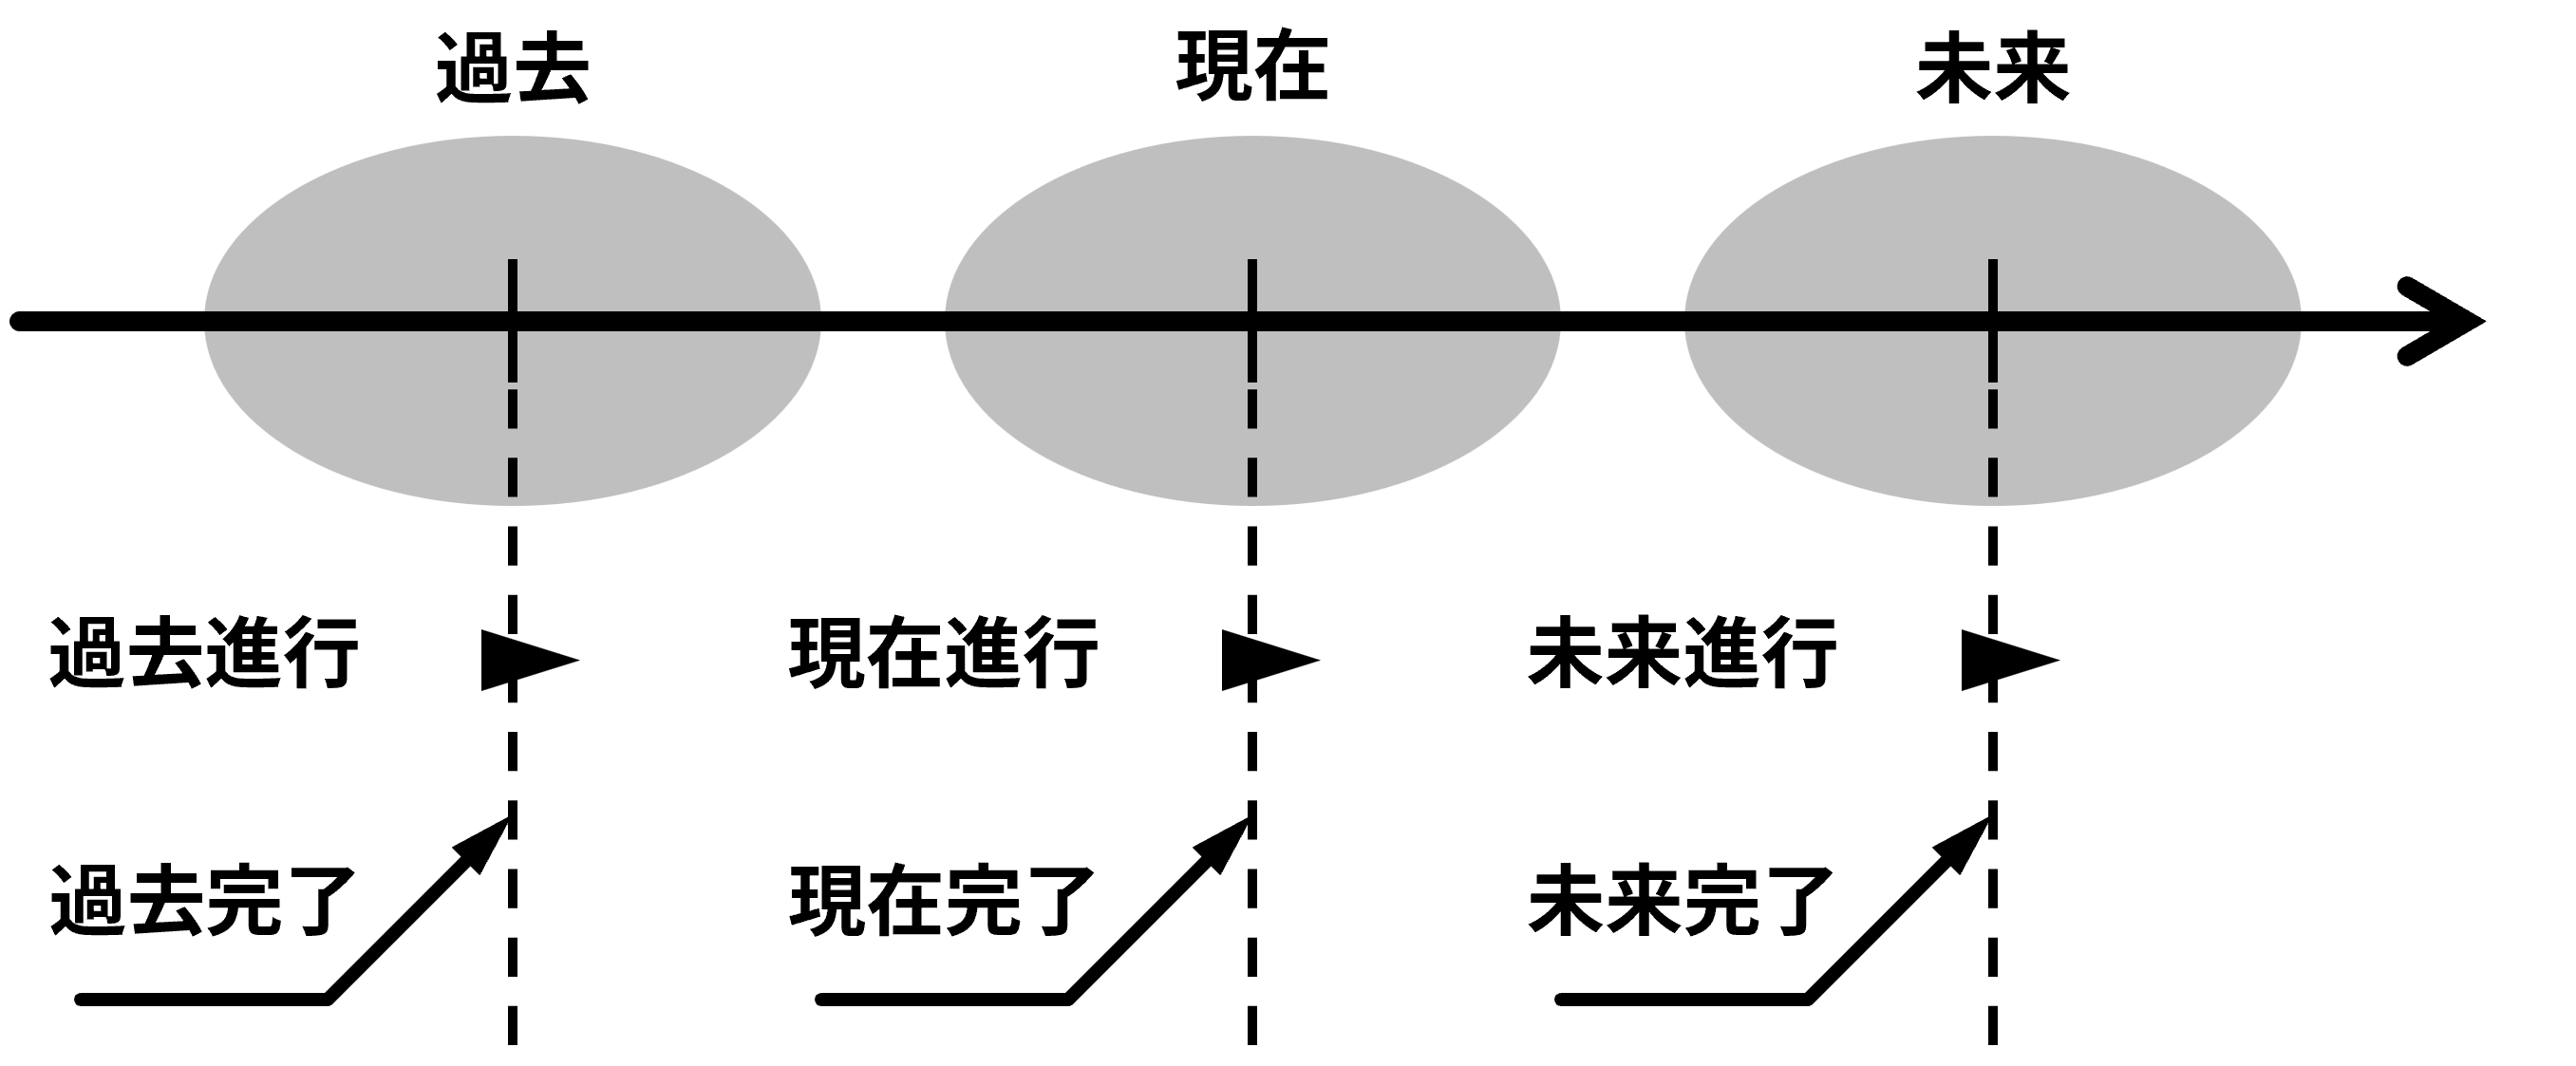
\includegraphics[width=100mm]{fig01.png}
\end{figure}

\subsubsection{現在・過去・未来}

単純な現在は、ざっくりと現在の時点付近のことを述べるのに使う。また、習慣などの反復的な行いや、普遍的な事実について述べるときにも使う。

単純な過去と未来についても、ざっくりとある過去の時点やある未来の時点付近のことを述べるのに使う。

\subsubsection{進行}

進行形は、ある時点で何かの動作や状態が継続しているときに使う。
現在進行形は自明に現在時点についての話だと自明にわかるが、過去進行形と未来進行形はどの時点で進行中なのかを特定させる必要がある。
たとえば、以下の例文を考える。

\begin{align}
  &I ~ am ~ playing ~ the ~ piano \text{.}\\
  &I ~ was ~ playing ~ the ~ piano ~ when ~ my ~ father ~ came ~ home \text{.}\\
  &I ~ will ~ be ~ playing ~ the ~ piano ~ when ~ my ~ father ~ comes ~ home ~ tomorrow \text{.}
\end{align}

どちらも「私はピアノを弾いている最中」であるという文章であるが、一つ目は現在進行形である一方で、二つ目は過去進行形、三つ目は未来進行形である。
後ろの二つでは「どのときに」ピアノを弾いている最中だったのかを示す必要があるため、「父が帰ってきたとき」「明日父が帰ってくるとき」というように過去や未来のどの時点かを特定する文言が入っている。
他にも「昨日の何時」などのように時間を指定する文言が入ることがある。
一方で、単に「昨日」や「先週」というような時間的に幅のある文言が入ることはない。
ちなみに、三つ目のwhen節について、「〇〇するとき」という副詞節のwhen節の中では、たとえ未来のことであっても未来形を使うことができない。
よって、単に現在形での表現になっている。

\subsubsection{完了}

完了には、完了・結果、経験、継続の三つの使われ方がある。
どれにも共通していることとしては、「ある時点から見たときの、過去からある時点までの時間の流れ」に着目している点である。
また進行形と同様に、現在完了は現在までについての話だと自明にわかるが、過去完了や未来完了はどの時点までの話なのかを特定させる必要がある。

\paragraph{完了・結果}\quad\\

完了・結果は、「ある時点でVしたところだ」(完了)あるいは「Vしてしまった」(結果)という意味である。

\begin{align}
  &I ~ have ~ finished ~ my ~ homework \text{.}\\
  &I ~ had  ~ finished ~ my ~ homework ~ by ~ dinner ~ yesterday \text{.}\\
  &I ~ will ~ have ~ finished ~ my ~ homework ~ by ~ dinner ~ tomorrow \text{.}
\end{align}

一つ目の文章なら「現時点で」、二つ目と三つ目の文章なら「昨日(明日)の夕食までに」宿題を終わらせているという文章になる。

特に完了の文脈でよく使われる単語を以下に示す。

\begin{table}[H]
  \centering
  \begin{tabular}{ll}
    \hline
    \multicolumn{1}{c}{英語} & \multicolumn{1}{c}{日本語}\\
    \hline \hline
    just & ちょうどVした \\
    already & 既にVした \\
    $not \sim yet$ & まだVしてない \\
    \hline
  \end{tabular}
\end{table}

「してしまった」という訳もある通り、単なる過去形の文章に後ろめたい気分を付け加えるため完了形にするという場合もある。
また、行くという意味で$gone$を用いたときは結果として捉えられ、「もう行ってしまった(ので結果ここにはいない)」という意味合いになる。
一方、行くという意味で$been$を用いたときは完了として捉えられ、「行ってきたところだ(行くという行為を完了した)」という意味合いになる。

\begin{equation}
  She ~ has ~ gone ~ to ~ New ~ York \text{.}
\end{equation}

\begin{equation}
  She ~ has ~ just ~ been ~ to ~ New ~ York \text{.}
\end{equation}

\paragraph{経験}\quad\\

経験は、「ある時点でVしたことがある」という意味である。

\begin{align}
  &I ~ have ~ visited ~ France \text{.}\\
  &I ~ had ~ visited ~ France ~ as ~ of ~ three ~ years ~ ago \text{.}\\
  &I ~ will ~ have ~ visited ~ France ~ three ~ times ~ if ~ I ~ go ~ to ~ Paris ~ next ~ year \text{.}
\end{align}

一つ目の文章なら「現時点で」、二つ目の文章なら「三年前の時点で」、三つ目の文章なら「来年もしパリに行ったならばその時点で」フランスに行ったことがあるという文章になる。
ちなみに、三つ目のif節についても、when節と同様にたとえ未来のことであっても未来形を使うことができない。
よって、単に現在形での表現になっている。

特に経験の文脈でよく使われる単語を以下に示す。

\begin{table}[H]
  \centering
  \begin{tabular}{ll}
    \hline
    \multicolumn{1}{c}{英語} & \multicolumn{1}{c}{日本語}\\
    \hline \hline
    once & 一度 \\
    twice & 二度 \\
    n times & n回 \\
    before & 以前 \\
    never & 一度もVしたことがない\\
    ever & (疑問文で)今までに\\
    \hline
  \end{tabular}
\end{table}

$gone$は結果の意味合いを持つため、経験の意味合いで行くという動詞を使いたいときは$been$を用いる。
そうすることで、「行ったことがある」という意味にすることができる。

\begin{equation}
  She ~ has ~ been ~ to ~ New ~ York ~ before \text{.}
\end{equation}

\paragraph{継続}\quad\\

継続は、「ある時点以前から継続してVし続けている」という意味である。

\begin{align}
  &I ~ have ~ lived ~ Osaka ~ for ~ three ~ years \text{.}\\
  &I ~ had ~ lived ~ Osaka ~ for ~ three ~ years ~ last ~ month \text{.}\\
  &I ~ will ~ have ~ lived ~ Osaka ~ for ~ three ~ years ~ next ~ month \text{.}
\end{align}

一つ目の文章なら「現時点で」、二つ目の文章なら「先月の時点で」、三つ目の文章なら「来月の時点で」大阪に三年間住み続けているという文章になる。
継続の意味で使う動詞は、基本的に動作を表す動詞ではなく状態を表す動詞である点に注意。

特に継続の文脈でよく使われる単語を以下に示す。

\begin{table}[H]
  \centering
  \begin{tabular}{ll}
    \hline
    \multicolumn{1}{c}{英語} & \multicolumn{1}{c}{日本語}\\
    \hline \hline
    for & の期間 \\
    since & から \\
    \hline
  \end{tabular}
\end{table}

\paragraph{大過去(過去完了のみ)}\quad\\

大過去とは、過去のある時点よりもさらに前の時点を示すときに過去完了形を使うケースである。
完了・結果、経験、継続といった意味があるわけではなく、単に過去より過去(大過去)のことを表すために時制を変えているだけなので、訳出には特別影響しない。

\begin{equation}
  I ~ broke ~ a ~ pen ~ my ~ father ~ had ~ given ~ me \text{.}
\end{equation}

この文は「私は父からもらったペンを壊してしまった」という文章だが、「父からもらった」のは「ペンを壊した」時よりも過去の時点になるので、過去完了形が使われている。
ただ、二つの事柄の前後関係をはっきりさせるときは大過去を使うが、前後関係がわかりきっているときや、ほぼ同じタイミングであるときなどは、普通に過去形を二回使うので構わない。

\subsubsection{完了進行}

完了進行は、「その時点以前から継続してVし続けている」のを表すのに使う。
継続の意味の完了とほぼ同じだが、あちらは状態を表す動詞に対して使う時制である一方、こちらは動作を表わす動詞に対して使う時制である。

\begin{align}
  &I ~ have ~ been ~ studying ~ English ~ for ~ three ~ hours \text{.}\\
  &I ~ had ~ been ~ studying ~ English ~ for ~ three ~ hours ~ when ~ I ~ realized ~ that \text{.}\\
  &I ~ will ~ have ~ been ~ studying ~ English ~ for ~ three ~ hours ~ in ~ ten ~ minutes \text{.}
\end{align}

一つ目の文章なら「現時点で」、二つ目の文章なら「気づいたときには」、三つ目の文章なら「あと10分で」英語を三時間勉強し続けているという文章になる。
完了進行の文脈でよく使われる単語は、継続のものと同じである。

\subsection{各時制の表し方}

それでは、各時制について、どのような操作を行えばよいかを学ぶ。

\subsubsection{現在・過去・未来}

\begin{itemize}
  \item 過去\\
  動詞を過去形(Vp)にする。\\
  助動詞がある場合は助動詞を過去形にして動詞を原形に戻す。
  \item 現在\\
  動詞を現在形にする。\\
  助動詞がある場合は助動詞を現在形にして動詞を原形に戻す。\\
  三単現の場合は動詞を三単現の形に活用する。\\
  助動詞がある場合は助動詞を三単現の形に活用して動詞を原形に戻す。\\
  (ただし、三単現の活用がある助動詞は$do \rightarrow does$のみなので、ほとんど考える必要はない)
  \item 未来\\
  助動詞willを挿入する。
\end{itemize}

\subsubsection{進行・完了}

\begin{itemize}
  \item 進行\\
  まず動詞を現在分詞(Ving)に変化させる。\\
  ただ、そうなると活用によって動詞が形容詞となるので、文から動詞がなくなる。\\
  そこで、現在分詞の直前に動詞としてbe動詞を挿入する。\\
  \begin{equation}
    V \rightarrow be + Ving
  \end{equation}
  \item 完了\\
  まず動詞を過去分詞(Vpp)に変化させる。\\
  ただ、そうなると活用によって動詞が形容詞となるので、文から動詞がなくなる。\\
  そこで、現在分詞の直前に動詞としてhaveを挿入する。\\
  \begin{equation}
    V \rightarrow have + Vpp
  \end{equation}
  \item 完了進行\\
  完了と進行の合わせ技をする。\\
  進行形への変化をしてから完了形への変化をすることで完了進行形となる。\\
  \begin{align}
    \begin{aligned}
      V & \rightarrow be + Ving\\
        & \rightarrow have + been + Ving
    \end{aligned}
  \end{align}
\end{itemize}

\subsubsection{複合時制}

現在・過去・未来の3種類と、単純(進行でも完了でもない普通の時制)・進行・完了・完了進行の4種類で、$3 \times 4 = 12$種類の時制が存在する。
それぞれの変形がどのようになるかを以下の表でまとめる。

\begin{table}[h]
  \centering
  \begin{tabular}{clll}
    \hline
     & \multicolumn{1}{c}{過去} & \multicolumn{1}{c}{現在} & \multicolumn{1}{c}{未来}\\
    \hline \hline
    単純 & Vp & V & will V\\
    進行 & be(was/were) Ving & be(is/am/are) Ving & will be Ving\\
    完了 & had Vpp & have Vpp & will have Vpp\\
    完了進行 & had been Ving & have been Ving & will have been Ving\\
    \hline
  \end{tabular}
\end{table}

\subsubsection{文法上の注意点}

ここまで読んで教えてもらった知識と違うと感じる人もいるだろう。
学校教育でもインターネット上の情報でも、はたまた歴史ある辞書でも、完了形のhaveは助動詞として紹介されているからだ。
その代わりに、過去分詞になった動詞を準動詞と呼び動詞として働くものとしている。
これは、意味上の動詞を動詞として扱いたいという考えのもと作られたメソッドである。
当たり前だが、完了形だろうが進行形だろうが意味上の動詞はVのまま変化しない。
だから、過去分詞になったとしてもVppを動詞ライクなものとして扱いたいのだ。
しかし、ここでは分詞になったらもはや動詞ではなくなるという考えのほうを重視し、形式上の動詞としてhaveを置くことにした。
もちろん、この考えにもデメリットがある(後述の疑問形の作り方の部分に影響する)ので、どちらの発想も頭に入れておくに越したことはない。
ややこしい話なので、一旦は「とりあえず完了のhaveは動詞として考えるけど、助動詞的な役割をすることもあるんだな」と思っておいてもらえるとありがたい。


